\documentclass[11pt]{article}
 \usepackage{amsmath}
 \usepackage{amssymb}
 \usepackage{amsthm}
 \usepackage{graphicx}
 \usepackage{float}
 \newtheorem{thm}{Theorem}
 \newtheorem{deftn}{Definition}
\title{Van Der Pol Equation}
\author{Siddharth Hari Nair\\130010011\thanks{This document has been prepared as part of the requirements for the first course project}}
\date{}
\begin{document}
\maketitle
\begin{abstract}
This document presents a study on the behaviour of the solutions to the Van der Pol oscillator. Post the introduction, the equilibria of the system are obtained and characterized followed by representative simulations of the various solutions of the equation.
\end{abstract}
\section{Introduction}
The Van der Pol equation, name after telecommunications pioneer Balthazar Van der Pol (1889-1959), is a second-order nonlinear differential equation most commonly examined in the field of nonlinear oscillations. Th equation models the oscillating charge of the Van der Pol oscillator, a simple circuit with a parallel capacitor, charge source and inductor in series with a tunnel diode.
\par
The key feature  of the Van der Pol oscillator is that its damping may be positive or negative in relation to the current amplitude of the oscillations. Specifically, larger oscillations are positively damed to become smaller, while smaller oscillations are negatively damped to become larger. all tending toward the same range of dynamic behaviour. In fact, all forms of the unforced Van der Pol oscillator tend toward a single stable limit cycle for their oscillations. For the purposes of telecommunications, circuits providing this functionality are useful in their ability to make both loud and quiet signals more easily perceived by the recipient. The only other equilibrium reached by the Van der Pol equation is the unstable  fixed point with zero amplitude and zero velocity, since a circuit containing no charge or charge source will see no oscillation; however, even the slightest bump of the circuit will eventually create a signal following the expected limit cycle.
\section{Dynamics}
The standard form of the Van der Pol equation is given by
\begin{equation}\label{vdp}
\ddot{x}+\mu(x^2-1)\dot{x}+x=0
\end{equation}
The equation can be physically construed as an oscillator with a linear spring force and a nonlinear damping force. The following analysis assumes that the factor $\mu >0$. On closer inspection of the equation, it can be seen that when $|x| <1$, the damping force is negative, i.e, reinforces the motion. For $|x| >1$, the damping force is positive and decays the motion. Such behaviour suggests the possibility of an oscillation, in which the system starts at small $x$, is driven to a large $x$ by the amplification, and is then damped back to small $x$.
\section{Equilibria and stability}
On writing \eqref{vdp} in state space form, the dynamics are 
\begin{align}\label{ss}
\dot{x}_1&=x_2 \nonumber \\
\dot{x}_2&=-x_1-\mu(x^2_1-1)x_2
\end{align}
where $x_1=x$ and $x_2=\dot{x}$. It is easy to see that the point $[\ x_1\ x_2\ ]^T\ =\ [\ 0\ 0\ ]^T$ is an equilibrium for the above dynamics. 
\subsubsection*{Case 1: $\mu >0$}
On linearizing the above dynamics about the equilibrium, we obtain the following linear system.
\begin{equation}
\begin{bmatrix}\dot{x}_1\\\dot{x}_2\end{bmatrix}=\begin{bmatrix} 0 & 1 \\-1 & \mu\end{bmatrix}\begin{bmatrix}x_1\\x_2\end{bmatrix}
 \end{equation}
 The eigenvalues of the above system are $\frac{\mu+\sqrt{\mu^2-4}}{2}$ and $\frac{\mu-\sqrt{\mu^2-4}}{2}$ both of which are positive for $\mu >0$. Hence, the  equilibrium is unstable (see Lyapunov's Indirect method \cite{slotine}). On closer inspection, for $0<\mu<2$, the eigenvalues are complex and on the right half of the complex plane. Therefore, the behaviour of the solutions local to the equilibrium point resembles that of an unstable spiral.
\subsubsection*{Case 2: $\mu<0$}
To analyze the stability of the equilibrium, we consider the following Lyapunov function candidate $$V = x^2_1 +x^2_2 $$
Taking its time derivative along the state trajectories, we obtain $$\dot{V}=-2\mu(x^2_1-1)x^2_2$$ which is negative semidefinite in the region $D=\left\{(x_1,x_2)\ |\  x^2_1 \leq 1\right\}$. Hence, the equilibrium is stable for any initial condition in $D$ (see Lyapunov's Direct method \cite{slotine}).
\subsection*{Limit Cycle}
\begin{deftn}[Li\'enard Equation]
Let $f$ and $g$ be two continuously differentiable functions on $\mathbb{R}$ with $f$ and $g$ as even and odd functions respectively. Then the second order differential equation of the form $$ \ddot{x}+f(x)\dot{x}+g(x)=0$$ is called a Li\'enard equation \cite{belur}.
\end{deftn}
We observe that the Van der Oscillator is a Li\'enard equation with the even function $f(x)=\mu(x^2-1)$ and odd function $g(x)=x$.  The next theorem further characterizes such equations to establish the existence of limit cycles.
\begin{thm}[Li\'enard's Theorem]
A Li\'enard system has a unique and stable limit cycle surrounding the origin if it satisfies the following properties
\begin{itemize}
\item $g(x) >0$ for all $x >0$
\item $f(x)<0$ for $0<x<p$ and $f(x)>0$ and monotonic for $x>p$
\end{itemize}
\end{thm} 
The proof is omitted and deferred to \cite{Lienard}.\\
We observe that the Van der Pol oscillator qualifies the requirements of theorem and thus possesses a unique and stable limit cycle. 
\section{Simulations}
We obtain numerical solutions to the van der pol equation under,
\begin{table}[H]
\centering
\begin{tabular}{| c | c |}
\hline
 Damping Coeffecient & Initial Conditions \\
 &\\\hline
 -0.1 & [1,0.5] \\\hline
 5 & [3,0.5] \\\hline
 -0.05 & [2,0.5] \\\hline
 5 & [1,0.5] \\\hline
 3 & [-2.5,-2] \\\hline
 \end{tabular}
\caption{Solution Conditions}
\end{table}

\begin{figure}[H]
\centering
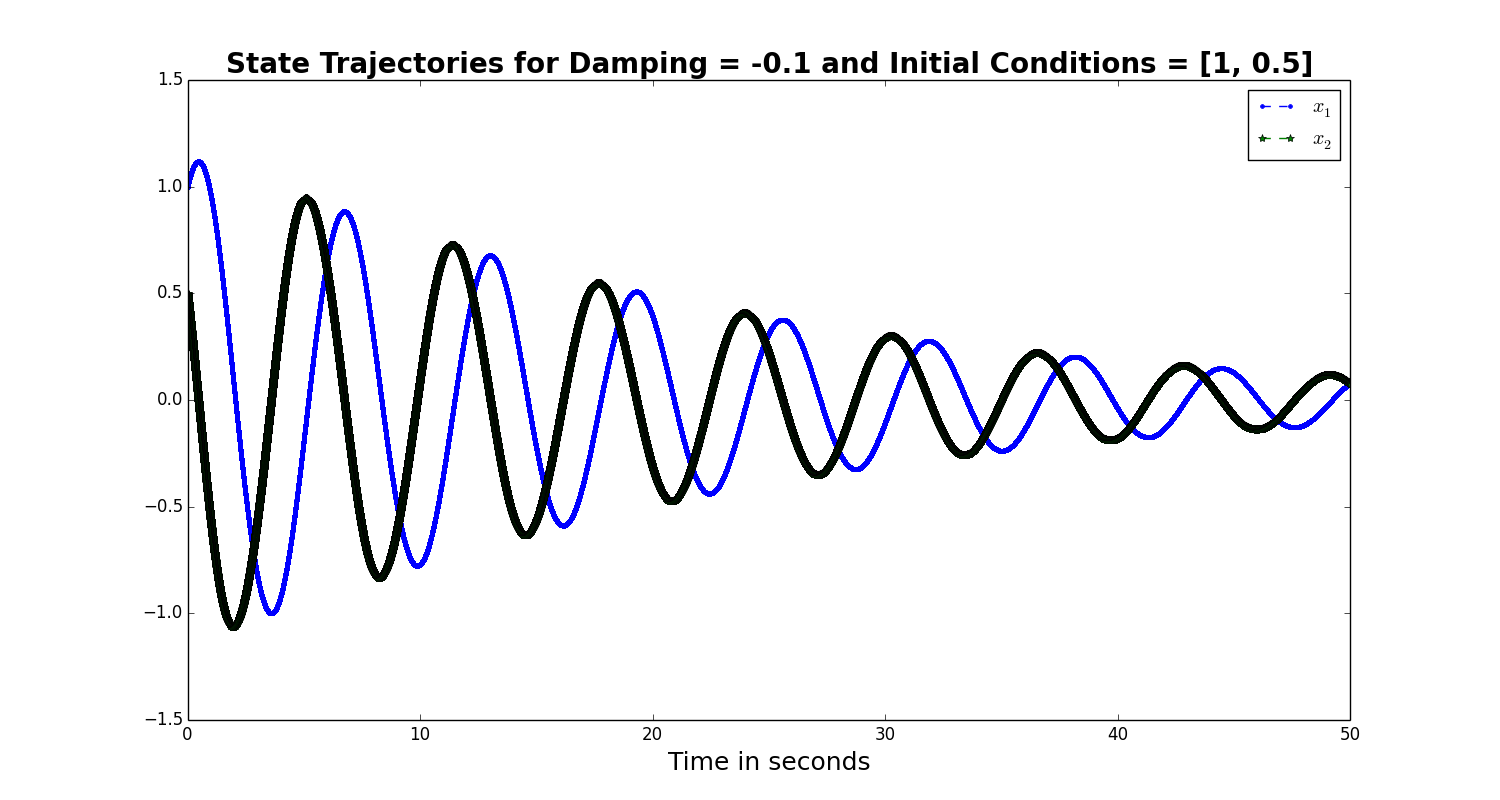
\includegraphics[scale=0.35]{vanderpol_trajectories0}
\end{figure}
\begin{figure}[H]
\centering
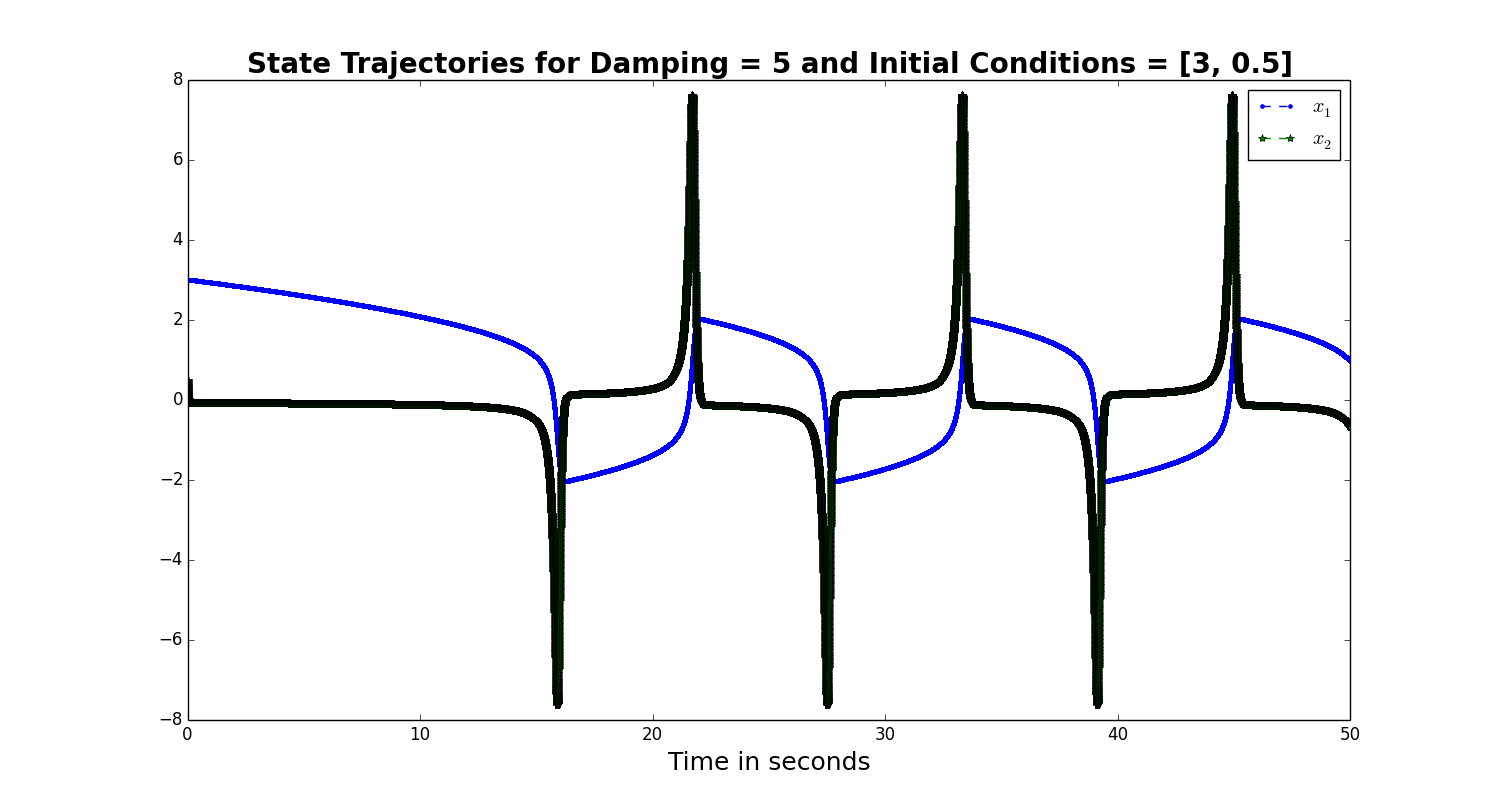
\includegraphics[scale=0.35]{vanderpol_trajectories1}
\end{figure}
\begin{figure}[H]
\centering
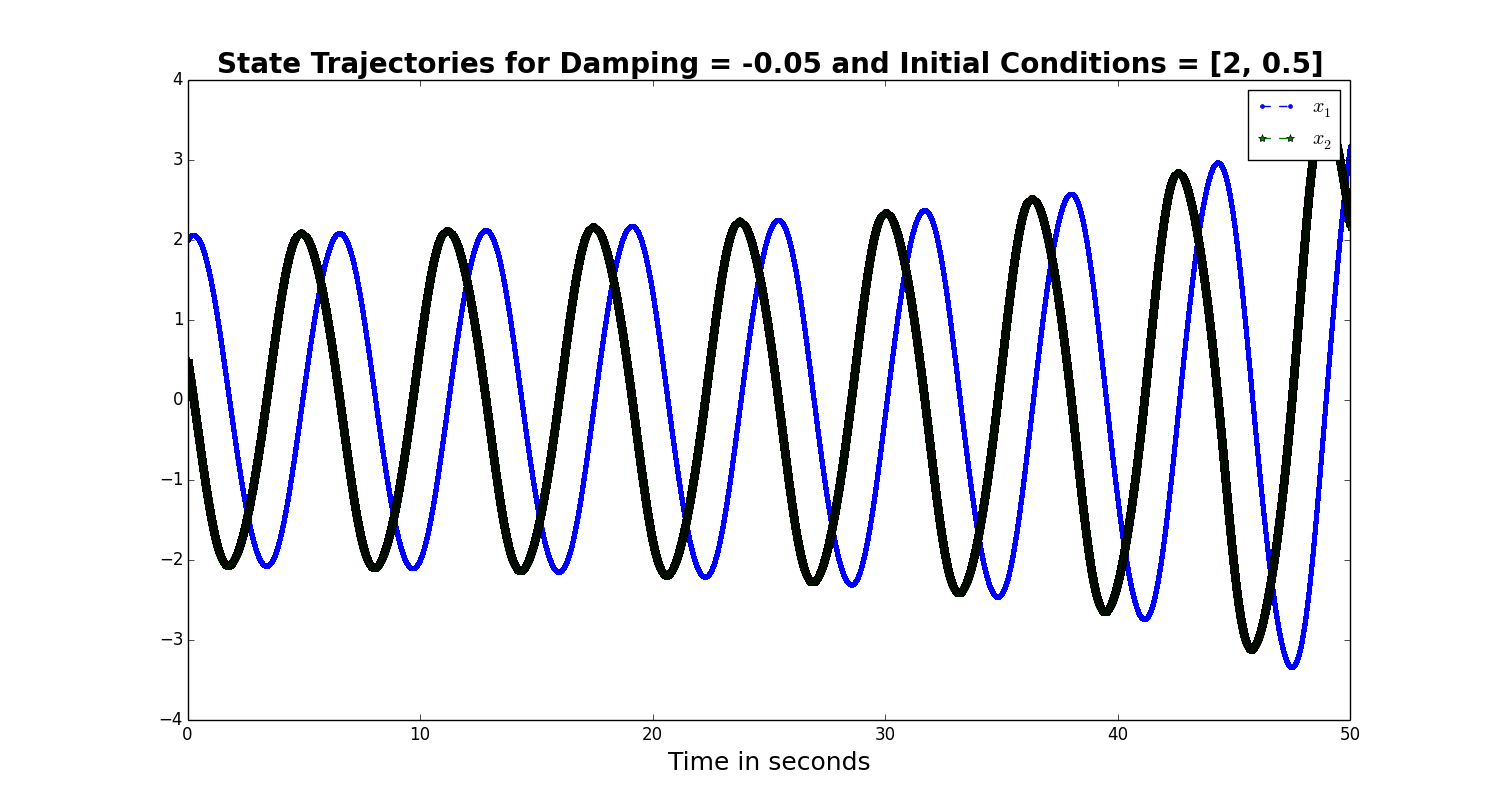
\includegraphics[scale=0.35]{vanderpol_trajectories2}
\end{figure}
\begin{figure}[H]
\centering
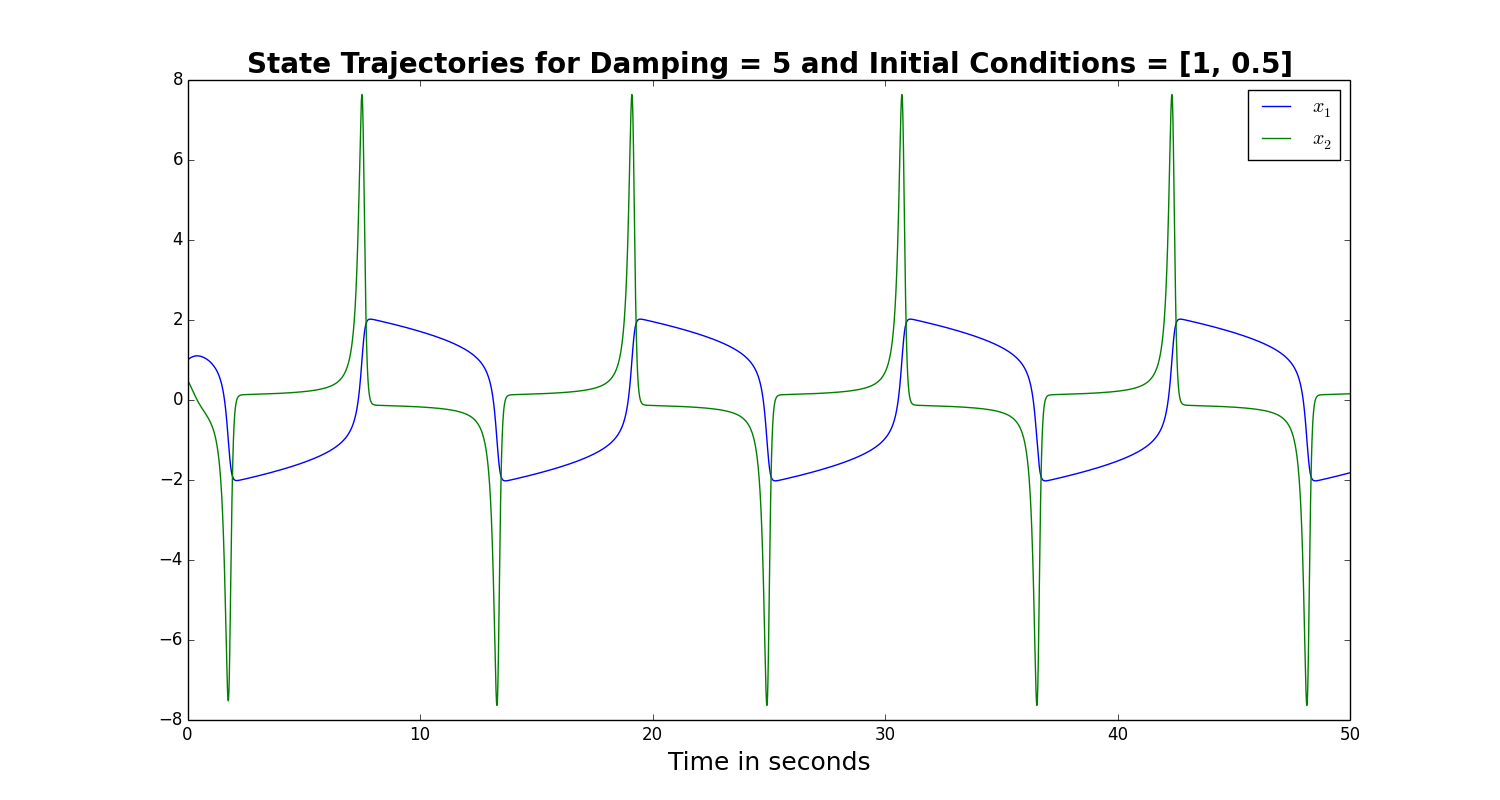
\includegraphics[scale=0.35]{vanderpol_trajectories3}
\end{figure}
\begin{figure}[H]
\centering
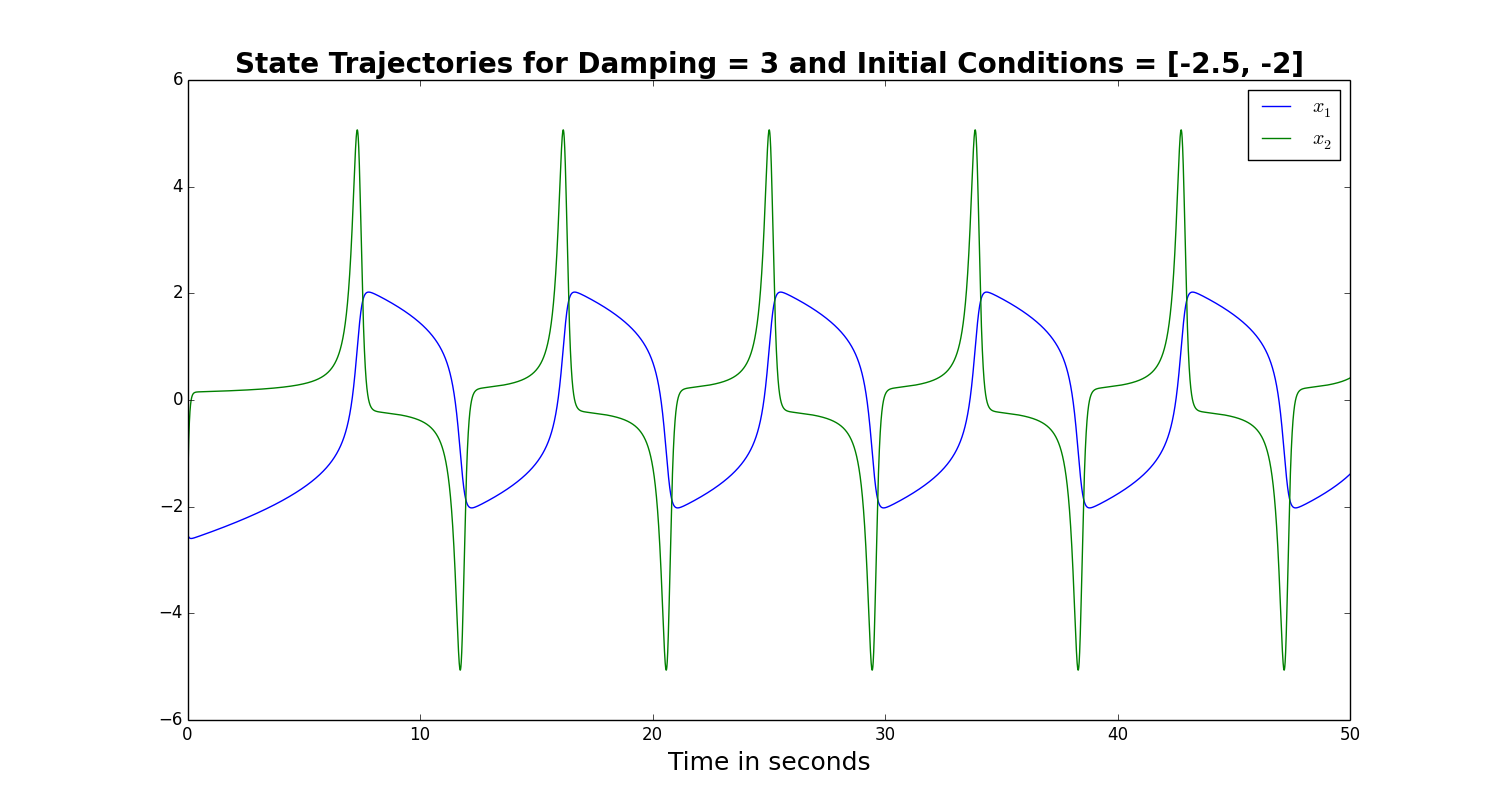
\includegraphics[scale=0.35]{vanderpol_trajectories4}
\end{figure}
\begin{figure}[H]
\centering
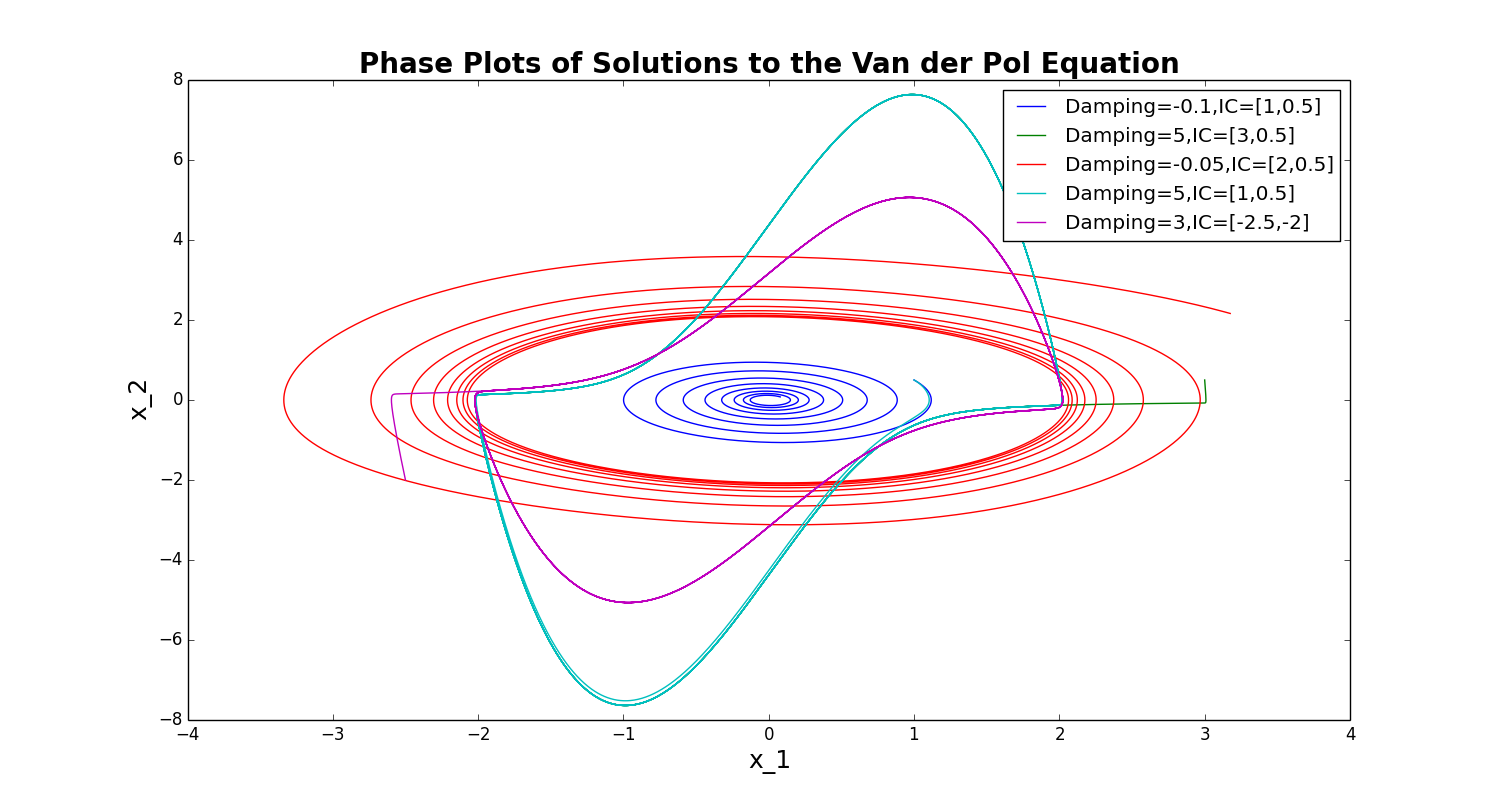
\includegraphics[scale=0.35]{vanderpol_equation}
\end{figure}
 \bibliographystyle{ieeetr}
 \bibliography{Ref}
\end{document}